\documentclass[crop=false,a4paper,oneside,11pt]{standalone}
\usepackage{a4wide,graphicx,fancyhdr,amsmath,amssymb,float,graphicx,color,geometry,xcolor,titlesec,colortbl,tabu}
\usepackage[parfill]{parskip}
\usepackage[nodayofweek]{datetime}
%----------------------- Macros and Definitions --------------------------

%fast change of things
\newcommand{\mysubject}{2IO70 DBL Embedded Systems}
\newcommand{\myassignment}{Group 12}

%\definecolor{titlepagecolor}{cmyk}{1,.60,0,.40}
%\definecolor{namecolor}{cmyk}{1,.50,0,.10}


\setlength\headheight{20pt}
\addtolength\topmargin{-10pt}
\addtolength\footskip{20pt}

% Define light and dark Microsoft blue colours
\definecolor{MSBlue}{rgb}{.204,.353,.541}
\definecolor{MSLightBlue}{rgb}{.31,.506,.741}
\arrayrulecolor{MSLightBlue}

% Set formats for each heading level

\titleformat*{\section}{\Large\bfseries\sffamily\color{MSBlue}}
\titleformat*{\subsection}{\large\bfseries\sffamily\color{MSLightBlue}}

%date format
\newdateformat{mydate}{\monthname[\THEMONTH] \THEYEAR}

\fancypagestyle{plain}{%
\fancyhf{}
\renewcommand{\headrulewidth}{0pt}
\renewcommand{\footrulewidth}{0pt}
}

\pagestyle{fancy}
\fancyhf{}
\fancyfoot[CO] {\thepage}
\renewcommand{\headrulewidth}{0pt}
\renewcommand{\footrulewidth}{0pt}


%--------------------------------- Text ----------------------------------
\setcounter{secnumdepth}{0}
\begin{document}

\section{Experimental Evaluation}

We ran all the tests in our experimental evaluation on a HP EliteBook 8570w with an Intel i7-3630QM CPU @ 2.40GHz and 8,00 GB RAM. To measure the amount of time and algorithm we start a timer in the code just before the part we want to test and we stop the timer right after the part stops. For testing the 2-position, 4-position and 1-slider algorithms we generated test cases with $5$ different distributions. These distributions are:
\begin{enumerate}
    \item Uniform. Points are randomly placed on a $10000$ by $10000$ plane.
    \item Clustered. Points are placed around $20$ randomly chosen points.
    \item H Clustered. Points are placed around $10$ randomly chosen $y$-coordinates.
    \item V Clustered. Points are placed around $10$ randomly chosen $x$-coordinates.
    \item Bounded. Points are randomly placed on a $1000$ by $1000$ plane.
\end{enumerate}

\subsection{2-position}
\subsubsection{Results}
The algorithm for the 2-position model is explained in detail in section 2.2. As a short recap, this algorithm has two phases: first we map all the collisions of every candidates of every single point, then we try to place the candidates that has least amount of collisions. For the experimental evaluation of the 2-position algorithm we used $2500$ different test cases with $500$ cases for each distribution. These test cases start with 100 points and increase with 100 points until 10000 points are reached. \\

\begin{figure}[h!]
 \centering
  \centerline{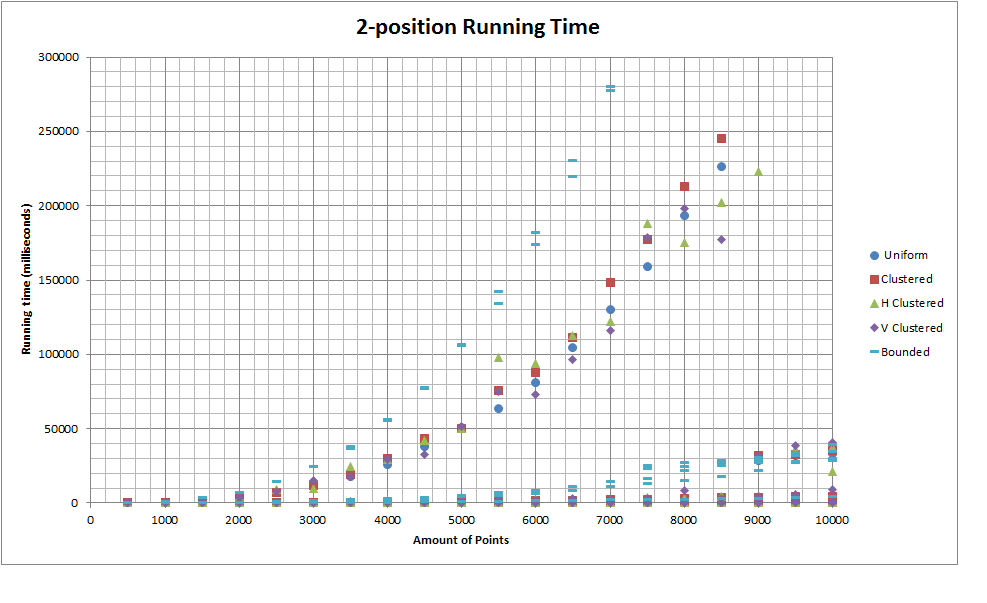
\includegraphics[scale = 0.5]{2PosRunningTime.png}}
  \caption{A graphic showing the running time of the 2-position algorithm}
 \end{figure}

\begin{figure}[h!]
 \centering
  \centerline{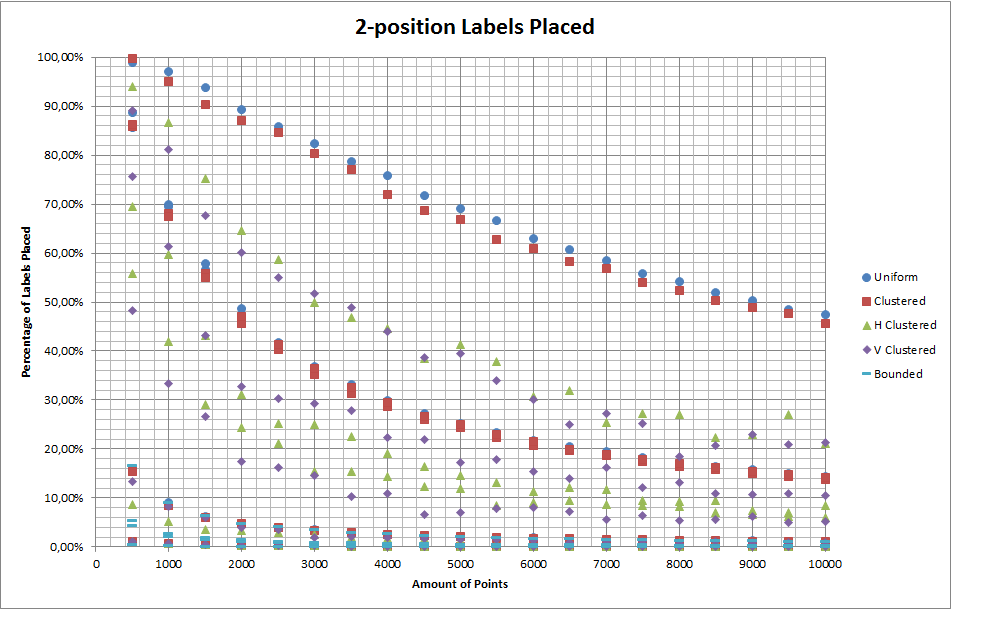
\includegraphics[scale = 0.5]{2PosLabelsPlaced.png}}
  \caption{A graphic showing the percentage of labels placed by the 2-position algorithm}
 \end{figure}
 
\subsubsection{Discussion}
As stated in section 2.2.1 the theoretical running time of the 2-position algorithm is $O(n^2)$. From figure ... we can see that the running time of most of the cases is close to their best case. This is because the amount of collisions of the candidates is small, so it will not take much time to map the collisions and it will take less time to place the labels. There are some cases that have higher running time than the others. And we can see from the figure that the practical worst case running time are close to the theoretical running time $O(n^2)$ as we explained before. \\
The worst cases of each distribution suddenly drops when the number of points reaches a specific amount. This is because in these cases, there are too many collisions. If we use the regular algorithm, the running time will become really high so it's not efficient. So in that case, we use greedy algorithm to place the labels. The running time will become lower and the solution is as optimal when using the regular algorithm since there are a lot of collisions.\\
Other than running time, we also look at the amount of placed labels of our algorithm. As we can see from figure ..., when the amount of points are small, the algorithm gives solutions with high percentage of placed labels. When the amount of points become higher, the percentage of placed labels will become lower. This is normal as the labels have the same height and the same width for the same type of distribution but with a higher amount of points. The reason why bounded cases have low solution is because all points are placed in a small area.\\

\subsection{4-position}
\subsubsection{Results}
The algorithm of 4-position model is explained in detail in section 2.2 It is basically the same as the algorithm of 2-position except it has two more possible label candidates. For the experimental evaluation of the 4-position algorithm we also used $2500$ different test cases with $500$ cases for each distribution. These test cases start with 100 points and increase with 100 points until 10000 points are reached.\\ 

 \begin{figure}[h!]
 \centering
 \centerline{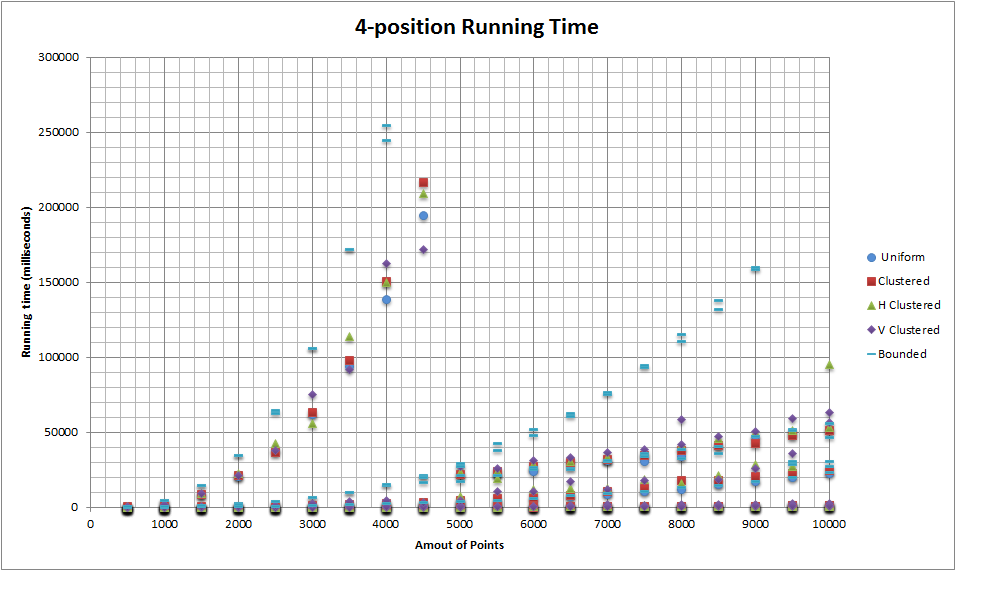
\includegraphics[scale = 0.5]{4PosRunningTime.png}}
 \caption{A graphic showing the Running Time of the 4-position algorithm}
 \end{figure}

 \begin{figure}[h!]
 \centering
  \centerline{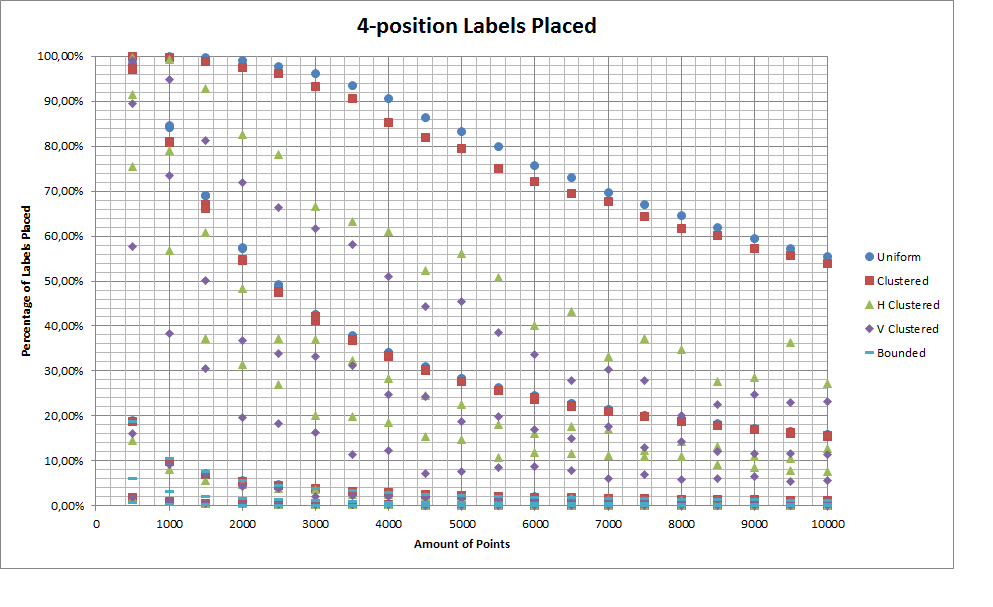
\includegraphics[scale = 0.5]{4PosLabelsPlaced.png}}
  \caption{A graphic showing the percentage of labels placed by the 4-position algorithm}
 \end{figure}
 
\subsubsection{Discussion}
As we stated in section 2.2.1, the algorithm for the 4-position model is nearly the same as the algorithm for the 2-position model. Hence the theoretical running time of the 4-position algorithm is also $O(n^2)$. In figure ..., it shows the running time of $2500$ different cases. As with the algorithm for the 2-position model, the running time for most of the cases is close to their best case. This is because the amount of collisions of the candidates is small, so it will not take much time to map the collisions and it will take less time to place the labels. We can see from the figure that the practical worst-case running time is close to the theoretical running time $O(n^2)$. \\
The running time of the worst cases of each distribution also suddenly drop when the number of points reaches a specific amount. This is because, in these cases, there are too many collisions and, as with the 2-position algorithm, we use a greedy algorithm to place the labels. But there are still some differences between the algorithm for the 2-position model and the 4-position model. The 4-position algorithm reverts to using the greedy algorithm faster than 2-position algorithm.(In around 4000 points) This is because, with the 4-position model, more collisions occur between candidates as there are more possible positions for a candidate to be in.\\
Other than running time, we also look at the amount of placed labels of our algorithm. As we can see from figure ..., when the amount of points are small, the algorithm gives solutions with high percentage of placed labels. When the amount of points become higher, the percentage of placed labels will become lower. This can be explained by the same situation in 2-position model. Compared to the result of 2-position algorithm, 4-position algorithm has higher solution in the percentage of placed labels since it has two more labels to place.\\

\subsection{1-slider}
\subsubsection{Results}
For the evaluation of the 1-slider algorithm we ran 500 test cases, 100 of each distribution. These test cases start with 500 points and increase with 500 points until 10000 points is reached. The 1-slider algorithm is explained in detail in section 2.3

 \begin{figure}[h!]
 \centering
 \centerline{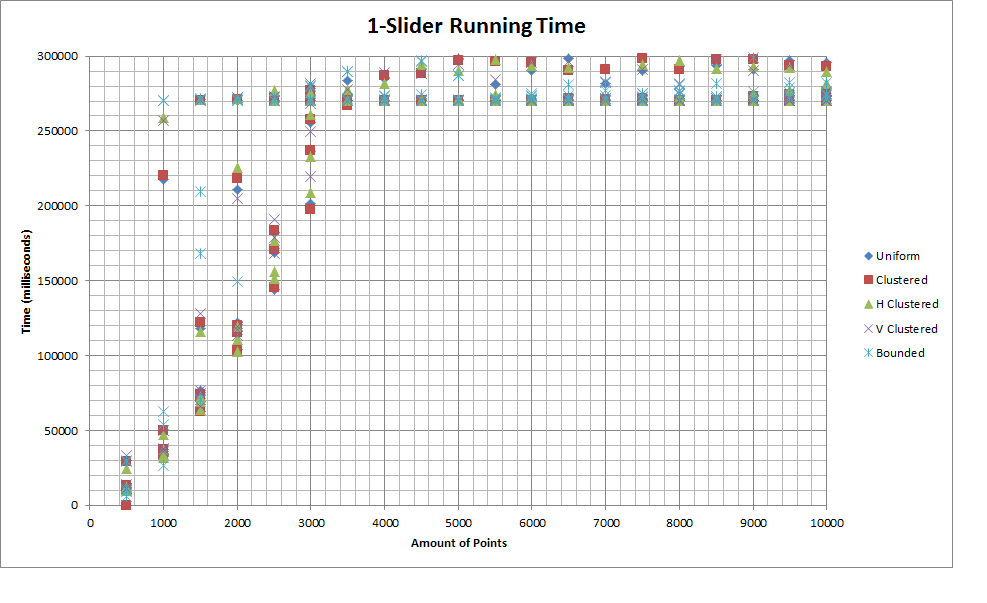
\includegraphics[scale = 0.65]{1slider.png}}
 \caption{A graphic showing the Running Time of the 1-slider algorithm}
 \end{figure}

 \begin{figure}[h!]
 \centering
  \centerline{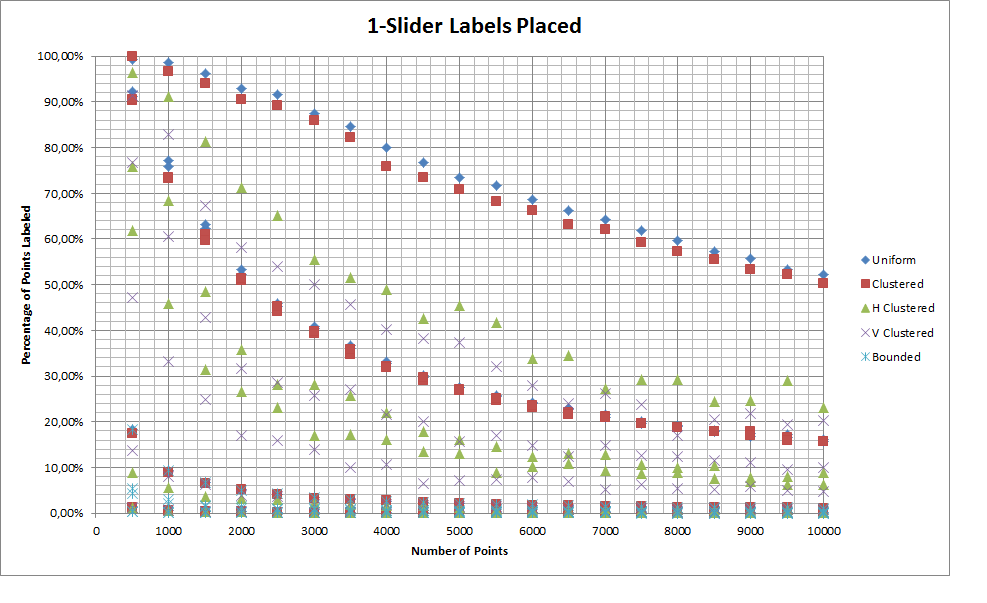
\includegraphics[scale = 0.65]{1sliderplaced.png}}
  \caption{A graphic showing the percentage of labels placed by the 1-slider algorithm}
 \end{figure}
 
\subsubsection{Discussion}
From section 2.3.9 we get that the theoretical running time of the 1-slider algorithm is $\theta(n^3)$. From the figure we can see that the practical running time matches the theoretical running time. The figure also shows that the running time of all the test cases plateaus after a certain amount of points is reached. This is because after 4.5 minutes has been reached we stop the algorithm and report the best solution found up to then.

\end{document}
